%%%%%%%%%%%%%%%%%%%%%%%%%%%%%%%%%%%%%%%%%
% Beamer Presentation
% LaTeX Template
% Version 1.0 (10/11/12)
%
% This template has been downloaded from:
% http://www.LaTeXTemplates.com
%
% License:
% CC BY-NC-SA 3.0 (http://creativecommons.org/licenses/by-nc-sa/3.0/)
%
% Modified by Jeremie Gillet in November 2015 to make an OIST Skill Pill template
%
%%%%%%%%%%%%%%%%%%%%%%%%%%%%%%%%%%%%%%%%%

%----------------------------------------------------------------------------------------
%	PACKAGES AND THEMES
%----------------------------------------------------------------------------------------

\documentclass{beamer}

\mode<presentation> {

\usetheme{Madrid}

\definecolor{OISTcolor}{rgb}{0.65,0.16,0.16}
\usecolortheme[named=OISTcolor]{structure}

%\setbeamertemplate{footline} % To remove the footer line in all slides uncomment this line
%\setbeamertemplate{footline}[page number] % To replace the footer line in all slides with a simple slide count uncomment this line

\setbeamertemplate{navigation symbols}{} % To remove the navigation symbols from the bottom of all slides uncomment this line
}
\setbeamertemplate{itemize items}[default]
\setbeamertemplate{enumerate items}[default]
\usepackage{graphicx} % Allows including images
\usepackage{booktabs} % Allows the use of \toprule, \midrule and \bottomrule in tables
\usepackage{textpos} % Use for positioning the Skill Pill logo
\usepackage{fancyvrb}
\usepackage{tikz}
\usepackage{hyperref}
\usepackage{listings}
\usepackage{color}

\definecolor{dkgreen}{rgb}{0,0.6,0}
\definecolor{gray}{rgb}{0.5,0.5,0.5}
\definecolor{mauve}{rgb}{0.58,0,0.82}

\lstset{frame=tb,
  language=python,
  aboveskip=3mm,
  belowskip=3mm,
  showstringspaces=false,
  columns=flexible,
  basicstyle={\small\ttfamily},
  numbers=none,
  numberstyle=\tiny\color{gray},
  keywordstyle=\color{blue},
  commentstyle=\color{dkgreen},
  stringstyle=\color{mauve},
  breaklines=true,
  breakatwhitespace=true,
  tabsize=3
}

\newcommand*{\lstitem}[1]{
  \setbox0\hbox{\lstinline{#1}}  
  \item[\usebox0]  
  % \item[\hbox{\lstinline{#1}}]
  \hfill \\
}

\usepackage[charsperline=65, theme=default-plain]{jlcode}
\usepackage[normalem]{ulem}
\DeclareRobustCommand\PICINTOC{}%


\newcommand\MYPICINTOC
  {\hfill
   \smash{\raisebox{-.74\height}{
\includegraphics[width=.39\textwidth]{if_meme.jpg}}}}

%----------------------------------------------------------------------------------------
%	TITLE PAGE
%----------------------------------------------------------------------------------------

\title[Mini Course]{Mini course: Julia} % The short title appears at the bottom of every slide, the full title is only on the title page
\subtitle{Lecture 3: IDEs, Data Structures, Coding Practices, and Algorithms}

\author{Gaston, Friederike,\\
        and Juan
} % Your name
\institute[OIST] % Your institution as it will appear on the bottom of every slide, may be shorthand to save space
{
Okinawa Institute of Science \\ 
and Technology \\ % Your institution for the title page
}
\date{March 5, 2021} % Date, can be changed to a custom date

\begin{document}

\setbeamertemplate{background}{
\includegraphics[width=\paperwidth]{background.png}} % Adding the background logo

\begin{frame}
\vspace*{1.4cm}
\titlepage % Print the title page as the first slide
\end{frame}

\setbeamertemplate{background}{} % No background logo after title frame

\addtobeamertemplate{frametitle}{}{% Adding the Skill Pill logo on the title screen after title frame
\begin{textblock*}{100mm}(.92\textwidth,-0.9cm)

\includegraphics[height=0.85cm]{julia.pdf}
\end{textblock*}}

\begin{frame}
    \addtocontents{toc}{\let\PICINTOC\string\MYPICINTOC}
    \tableofcontents
\end{frame}

\begin{frame}
\frametitle{Disclaimer}

When designing this Skill Pill, we assumed the following
\begin{itemize}
\item You have your own workflow in regards to which software and libraries you work with.
\item You have seen and are familiar with common data structures.
\item You know how to program and use programming as part of your daily work. 
\end{itemize}

As such, we have designed today's lesson so that you may begin using Julia in your work as soon as possible.

\end{frame}

\section{IDEs \& remote workflow \PICINTOC}

\begin{frame}
\frametitle{Workflow}
\centering

\includegraphics[width=\paperwidth,trim={7cm 5cm 4cm 5cm},clip]{IDEs&remote.png}
\end{frame}

\begin{frame}
\frametitle{Jupyter notebook}
\begin{itemize}
\item Step 1: Install Julia.
\item Step 2: Run ]add IJulia on Julia's REPL.
\item Step 3: Install Anaconda distribution
\item Step 4: Launch Jupyter lab/notebook from the Anaconda Navigator
\item Step 5: Create a new jupyter notebook with Julia kernel.
\end{itemize}
\end{frame}

\begin{frame}
\frametitle{Atom + Juno}
\begin{itemize}
\item Step 1: Install Julia, and Atom.
\item Step 2: Search in Atom for the packages: uber-juno, language-julia, julia-client, ink, and indent-detective.
\item Step 3: Restart and launch Julia in the REPL inside Atom. It will gather all remaining necessary packages.
\end{itemize}
\end{frame}

\begin{frame}
\frametitle{Visual Studio Code + Julia for VS}
\begin{itemize}
\item Step 1: Install Julia, and Visual Studio Code.
\item Step 2: Inside VSCode, go to extensions and search "julia". Install Julia for VSCode and restart.
\end{itemize}
\end{frame}

\begin{frame}
\frametitle{Remote connection to your workstation}

Depending on your workflow, you may want to have access to data, more computational resources, or just to avoid \sout{stressing out the crappy Macbooks} using your personal laptop for running research code.\\

On Jupyter notebook, this is done very easily. Make sure you have installed Jupyter notebook on both the local and remote computers.\\

Assuming you have access (via VPN) and know the IP of your workstation to run the following ...\\

\begin{block}{On remote host terminal:}
    \$ jupyter notebook --no-browser --port=8889
\end{block}

\end{frame}

\begin{frame}
\frametitle{Remote connection to your workstation}
In the \textbf{local host}, run the following in the terminal (cmd for Windows):\\

\begin{block}{To connect:}
\$ ssh -N -f -L localhost:8888:localhost:8889 user@remote\_host\_IP
\end{block}

Make sure to change \textit{user} to your real username in \textbf{remote host}, and change \textit{your$\_$remote$\_$host$\_$name} to your address of your working station. \\

\begin{block}{Example:}
\$ ssh -N -f -L localhost:8888:localhost:8889 gaston@10.2.80.145
\end{block}

Now open web browser and type:\\

\begin{block}{Web browser address bar:}
localhost:8888
\end{block}

\end{frame}

\begin{frame}
\frametitle{Remote connection to your workstation}
In Atom, the setup for remote workflow is very simple. 
\begin{itemize}
\item Install the following package inside Atom: \textbf{ftp-remote-edit}.
\item Go to Packages $\rightarrow$ Ftp-Remote-Edit $\rightarrow$ Toggle.
\item Right click on Remote tab $\rightarrow$ Edit server.
\item Name the server and input the necessary details.
\item To use tmux. Go to \textbf{julia-client} package settings $\rightarrow$ Remote settings $\rightarrow$ Use persistent tmux session. Also check that the command to execute Julia remotely is appropiate.
\item Start the remote server by going to Juno $\rightarrow$ Start Remote Julia Process.
\end{itemize}
\end{frame}

\begin{frame}
\frametitle{Remote connection to your workstation}
\centering
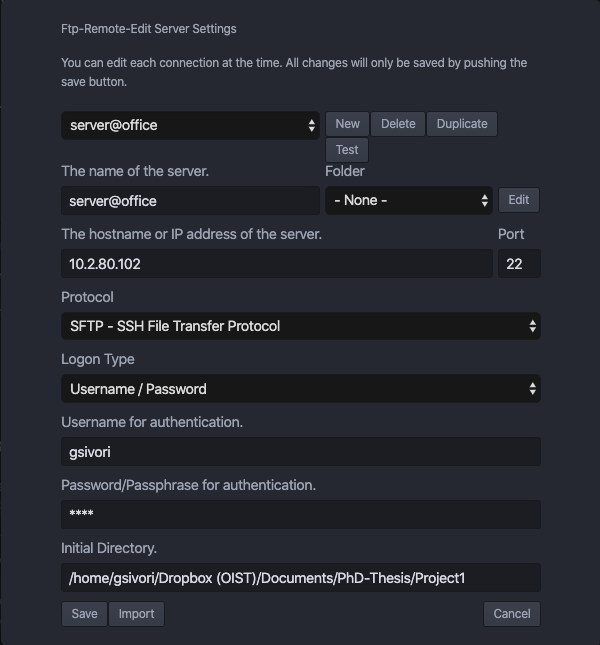
\includegraphics[width=0.55\paperwidth]{ftp-server-settings.png}
\end{frame}

\section{Data Structures}

\begin{frame}
\frametitle{Datastructures.jl}

\begin{columns}
\column{0.5\textwidth}
DataStructures.jl has the following data structures:
\begin{itemize}
\item Deque (based on block-list)
\item Stacks and Queues
\item Accumulators and Counters
\item Disjoint Sets
\item Binary Heap
\item Mutable Binary Heap 
\item Ordered Dicts and Sets
\item Dictionaries with Defaults
\item Trie (Tree)
\item Linked List
\item Sorted Dict, Multi-Dict and Set
\item Priority Queue
\end{itemize}
\pause
\column{0.5\textwidth}
All information regarding these Data Structures can be found Here: \url{ http://datastructuresjl.readthedocs.io/en/latest/index.html/}

\vspace{0.5cm}
All of these algorithms can be viewed with \texttt{@edit}. We'll use two more before hopping into algorithms: \texttt{Binary Trees} and \texttt{Priority Queues}
\end{columns}

\end{frame}

\begin{frame}[fragile]
\frametitle{Deque}
Based on contiguous blocks on memory. Similar to Julia's \textbf{Vector} implementation, but, as it grows, it avoids copying all values to a new Vector. 
\begin{lstlisting}[language=julia]
a = Deque{Int}()
isempty(a)          # test whether the dequeue is empty
length(a)           # get the number of elements
push!(a, 10)        # add an element to the back
pop!(a)             # remove an element from the back
pushfirst!(a, 20)   # add an element to the front
popfirst!(a)        # remove an element from the front
first(a)            # get the element at the front
last(a)             # get the element at the back
\end{lstlisting}
\end{frame}

\begin{frame}[fragile]
\frametitle{Circular Buffer}
A circular buffer of fixed capacity. New items are pushed to the back of the list, overwriting values circularly.
\begin{lstlisting}[language=julia]
cb = CircularBuffer{Int}(n) # n-element circular buffer
isfull(cb) # test whether the buffer is full
isempty(cb) # test whether the buffer is empty
empty!(cb) # reset the buffer
capacity(cb) # return capacity
size(cb) # same as length(cb)
push!(cb, 10) # overwrites front if full
pop!(cb) # remove the element at the back
pushfirst!(cb, 10) # overwrites back if full
popfirst!(cb)  # remove the element at the front
append!(cb, [1, 2, 3, 4]) # push at most last `capacity` items
convert(Vector{Float64}, cb) # convert items to type Float64
eltype(cb) # return type of items
fill!(cb, data) # grows the buffer up-to capacity
\end{lstlisting}
\end{frame}

\begin{frame}[fragile]
\frametitle{Stacks and Queues}
\begin{lstlisting}[language=julia]
s = Stack{Int}()  # create a stack
eltype(s)         # get the type of elements
push!(s, 1)       # push back a item
first(s)          # get an item from the top of stack
pop!(s)           # get and remove a first item
iterate(s::Stack) # Get a LIFO iterator of a stack
Iterators.reverse(s::Stack{T}) # Get a FILO iterator of a stack
s1 == s2 # check whether the two stacks are same
\end{lstlisting}
\begin{lstlisting}[language=julia]
q = Queue{Int}()
enqueue!(q, x)
x = first(q)
x = last(q)
x = dequeue!(q)
\end{lstlisting}
\end{frame}

\begin{frame}[fragile]
\frametitle{PriorityQueue}
A type of data structure that enqueues items by priority.
\begin{lstlisting}[language=julia]
julia> # Julia code
       pq = PriorityQueue();
julia> # Insert keys with associated priorities
       pq["a"] = 10; pq["b"] = 5; pq["c"] = 15; pq
PriorityQueue{Any,Any,Base.Order.ForwardOrdering} with 3 entries:
  "b" => 5
  "a" => 10
  "c" => 15
julia> # Change the priority of an existing key
       pq["a"] = 0; pq
PriorityQueue{Any,Any,Base.Order.ForwardOrdering} with 3 entries:
  "a" => 0
  "b" => 5
  "c" => 15
\end{lstlisting}
\end{frame}

\begin{frame}[fragile]
\frametitle{Red-black Tree}
A type of self-balancing binary tree that has an extra bit of information to make searching, inserting, and deleting operations with $O(log(n))$: \url{https://en.wikipedia.org/wiki/Red\%E2\%80\%93black_tree}
\begin{lstlisting}[language=julia]
julia> tree = RBTree{Int}();
julia> for k in 1:2:20
        push!(tree, k)
       end
julia> haskey(tree, 3)
true
julia> tree[4]
7
julia> for k in 1:2:10
        delete!(tree, k)
       end
julia> haskey(tree, 5)
false
\end{lstlisting}
\end{frame}

\section{Coding Practices}

\begin{frame}
\frametitle{Coding Practices}

Some recommended coding practices to consider with Julia.
\begin{itemize}
\item Measure performance with @time and check for memory allocations.
\item Break a function into multiple definitions (proper use of multiple dispatcher)
\item Consider variable type stability for compiler optimizations.
\item Access arrays in memory order (along columns in Julia) 
\item Pre-allocate output.
\item Use vectorized operation "@." for readability.
\item Consider using @views to look at big arrays.
\item Read through Profile.jl, BenchmarkingTools.jl, and Cthulu.jl packages for further optimizations and debugging.
\item Diferences with other languages: \url{https://docs.julialang.org/en/v1/manual/noteworthy-differences/}
\end{itemize}

\end{frame}

\begin{frame}[fragile]
\frametitle{@time}
Measure performance with @time. Notice how using global variable allocates unnecesary memory making this example run longer.
\begin{lstlisting}[language=julia]
julia> x = rand(1000);
julia> function sum_global()
           s = 0.0
           for i in x
               s += i
           end
           return s
       end;
julia> @time sum_global()
  0.017705 seconds (15.28 k allocations: 694.484 KiB)
496.84883432553846
julia> @time sum_global()
  0.000140 seconds (3.49 k allocations: 70.313 KiB)
496.84883432553846
\end{lstlisting}
\end{frame}

\begin{frame}[fragile]
\frametitle{@time}
Compared to passing it as an argument:

\begin{lstlisting}[language=julia]
julia> x = rand(1000);
julia> function sum_arg(x)
           s = 0.0
           for i in x
               s += i
           end
           return s
       end;
julia> @time sum_arg(x)
  0.007701 seconds (821 allocations: 43.059 KiB)
496.84883432553846
julia> @time sum_arg(x)
  0.000006 seconds (5 allocations: 176 bytes)
496.84883432553846
\end{lstlisting}
\end{frame}

\begin{frame}[fragile]
\frametitle{Break function in many definitions depending input}
\begin{lstlisting}[language=julia]
using LinearAlgebra
function mynorm(A)
    if isa(A, Vector)
        return sqrt(real(dot(A,A)))
    elseif isa(A, Matrix)
        return maximum(svdvals(A))
    else
        error("mynorm: invalid argument")
    end
end
\end{lstlisting}
This is better:
\begin{lstlisting}[language=julia]
norm(x::Vector) = sqrt(real(dot(x, x)))
norm(A::Matrix) = maximum(svdvals(A))
\end{lstlisting}
\end{frame}

\begin{frame}[fragile]
\frametitle{Consider variable type}
\begin{lstlisting}[language=julia]
function foo()
    x = 1
    for i = 1:10
        x /= rand()
    end
    return x
end
\end{lstlisting}
\begin{lstlisting}[language=julia]
function foo()
    x::Float64 = 1.0 / rand()
    for i = 2:10
        x /= rand()
    end
    return x
end
\end{lstlisting}
\end{frame}

\begin{frame}[fragile]
\frametitle{Access arrays in memory order}
Multi-dimensional arrays are stored in column-major order (arrays are stacked one column at a time).
\begin{lstlisting}[language=julia]
julia> x = [1 2; 3 4]
2×2 Array{Int64,2}:
 1  2
 3  4
julia> x[:]
4-element Array{Int64,1}:
 1
 3
 2
 4
\end{lstlisting}
A rule of thumb to keep in mind is that with column-major arrays, the first index changes most rapidly. Looping will be faster if the inner-most loop index is the first to appear in a slice expression. 
\end{frame}

\begin{frame}[fragile]
\frametitle{Pre-allocate output}
If your function returns an Array or some other complex type, it may have to allocate memory. Unfortunately, often times allocation and its converse, garbage collection, are substantial bottlenecks. Compare this:
\begin{lstlisting}[language=julia]
julia> function xinc(x)
           return [x, x+1, x+2]
       end;
julia> function loopinc()
           y = 0
           for i = 1:10^7
               ret = xinc(i)
               y += ret[2]
           end
           return y
       end;
\end{lstlisting}
\end{frame}

\begin{frame}[fragile]
\frametitle{Pre-allocate output}
To this:
\begin{lstlisting}[language=julia]
julia> function xinc!(ret::AbstractVector{T}, x::T) where T
           ret[1] = x
           ret[2] = x+1
           ret[3] = x+2
           nothing
       end;
julia> function loopinc_prealloc()
           ret = Vector{Int}(undef, 3)
           y = 0
           for i = 1:10^7
               xinc!(ret, i)
               y += ret[2]
           end
           return y
       end;
\end{lstlisting}
\end{frame}

\begin{frame}[fragile]
\frametitle{Pre-allocate output}
This changes a lot.
\begin{lstlisting}[language=julia]
julia> @time loopinc()
  0.529894 seconds (40.00 M allocations: 1.490 GiB, 12.14% gc time)
50000015000000
julia> @time loopinc_prealloc()
  0.030850 seconds (6 allocations: 288 bytes)
50000015000000
\end{lstlisting}
\end{frame}

\begin{frame}[fragile]
\frametitle{Use vectorized operation for readability}
Using $.$ for broadcast opearation messes up readability. Use "@." for vectorized operations.
\begin{lstlisting}[language=julia]
julia> f(x) = 3x.^2 + 4x + 7x.^3;

julia> fdot(x) = @. 3x^2 + 4x + 7x^3
\end{lstlisting}
If x is an Array, fdot(x) will have significantly faster performance. 
\end{frame}

\begin{frame}[fragile]
\frametitle{Consider @views to look into slices of big arrays}
\begin{lstlisting}[language=julia]
julia> x = rand(10^6);

julia> fcopy(x) = sum(x[2:end-1]);

julia> @views fview(x) = sum(x[2:end-1]);

julia> @time fcopy(x);
  0.003051 seconds (7 allocations: 7.630 MB)

julia> @time fview(x);
  0.001020 seconds (6 allocations: 224 bytes)
\end{lstlisting}
\end{frame}


\section{Algorithms}

\begin{frame}
\frametitle{Algorithms in Julia}
\begin{block}{Exercise}
\textbf{Implement your favorite algorithm in Julia}
\end{block}

I will be coding the Lorentz Attractor as an example.
Lorentz function given by:
\begin{gather*} 
   \frac{dx}{dt} = \sigma (y - x) \\
   \frac{dy}{dt} = x (\rho - z) - y \\
   \frac{dz}{dt} = xy - \beta z
\end{gather*} 
Solve this for $t=1:150$. Initial conditions $[1,1,1]$. $\sigma = 10, \rho = 28, \beta = 8/3$.
\end{frame}

\begin{frame}
\frametitle{The end of this mini course!}

\Huge{Thanks for joining us!}

\end{frame}

\end{document}
